\documentclass[12pt, a4paper]{article}

\usepackage[left=1.5cm, right=1.5cm, top=2cm, bottom=2cm, bindingoffset=0cm, headheight=15pt]{geometry}
\usepackage{fancyhdr}
\usepackage[russian]{babel}
\usepackage{amsmath}
\usepackage{libertine}
\usepackage{graphicx}
\usepackage{amsmath}
\usepackage{amsthm}

\setmainfont{Linux Libertine}

\pagestyle{fancy}
\chead{Алгоритмы и структуры данных, задача 6.6}
\cfoot{Михайлов Максим, M3137}

\begin{document}

\subsection*{Условие}

Покажите, что если взять обычное дерево поиска без всяких балансировок и добавлять в него элементы в порядке убывания $y$, то получится декартово дерево.

\subsection*{Решение}

Докажем по индукции по числу вершин в дереве.
\begin{proof}
    \begin{description}
        \item[База:] \hfill \\ $1$ вершина --- любое дерево из одной вершины есть дерево поиска.
        \item[Переход:] \hfill \\ Есть декартово дерево с $n$ вершинами, докажем, что добавление еще одной вершины с ключом $y_{n+1} \leq y_i \ \ \forall i\in[1\ldots n]$ не нарушает ни инвариант по ключам $X$, ни по $Y$.
        
        Т.к. мы строим дерево поиска, то условие на ключи $X$ не нарушается. Кроме того, новая вершина подвесится к некоторому листу, поэтому для сохранения инварианта по $Y$ достаточно, чтобы $y_{n+1}\leq y_k$, где $k$ --- вершина, к которой подвешивается новая вершина. Это верно, потому что элементы добавляются в порядке убывания $y$.
 
        \begin{figure}[h]
            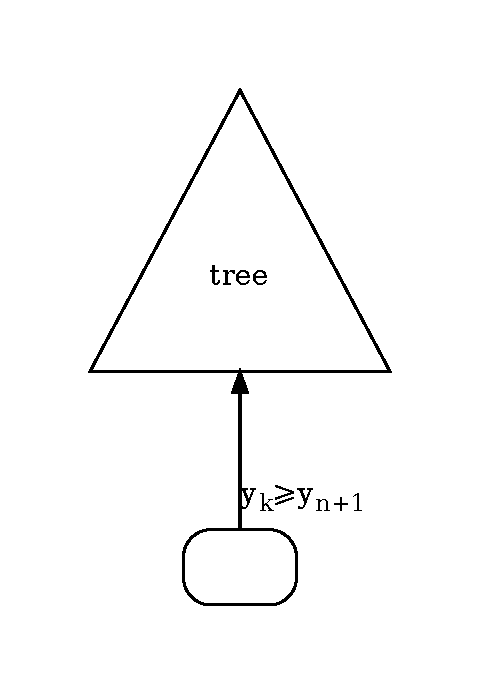
\includegraphics[scale=0.7]{add.pdf}
            \centering
        \end{figure}
    \end{description}
\end{proof}

\end{document}